\usetikzlibrary{shapes.geometric, arrows.meta, positioning, calc}
\tikzset{
  input/.style = {rectangle, draw=blue!70, fill=blue!10, thick, minimum height=1.2cm, minimum width=3.2cm},
  process/.style = {rectangle, draw=green!60!black, fill=green!10, thick, minimum height=1.2cm, minimum width=3.2cm},
  output/.style = {rectangle, draw=red!70, fill=red!10, thick, minimum height=1.2cm, minimum width=3.4cm},
  arrow/.style = {thick, -{Latex[length=3mm]}}
}

\centering
  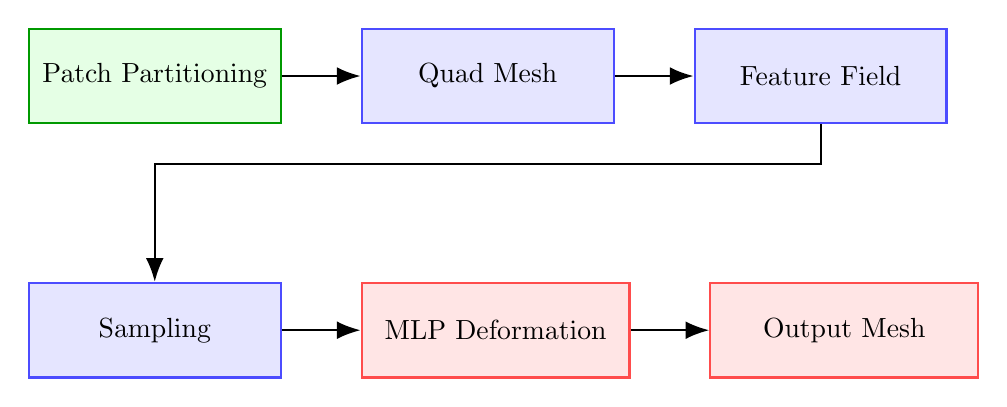
\begin{tikzpicture}[node distance=1cm and 1cm]

    % First row: one process + two input nodes
    \node[process] (partition) at (0,0) {Patch Partitioning};
    \node[input, right=of partition] (quadmesh) {Quad Mesh};
    \node[input, right=of quadmesh] (featurefield) {Feature Field};

    % Second row: three output nodes
    \node[input, below=2cm of partition] (sampling) {Sampling};
    \node[output, right=of sampling] (mlp) {MLP Deformation};
    \node[output, right=of mlp] (render) {Output Mesh};

    % Arrows top row
    \draw[arrow] (partition) -- (quadmesh);
    \draw[arrow] (quadmesh) -- (featurefield);

    % Arrows to second row
    \draw[arrow] (featurefield.south) -- ++(0,-0.5) -| (sampling.north);
    \draw[arrow] (sampling) -- (mlp);
    \draw[arrow] (mlp) -- (render);

  \end{tikzpicture}
  \vspace{-0.5em}
  \caption{Schematic of the processing pipeline. The input data undergoes patch partitioning and mesh structuring, followed by feature extraction. These are further processed through sampling and deformation stages to produce the final output mesh.}
\label{fig:teaser}
